\documentclass{beamer}
\usepackage{hyperref}
\usepackage{caption}
\usepackage[T1]{fontenc}
\usepackage[utf8]{inputenc}
\usepackage{lmodern}
\usepackage[english]{babel}
\linespread{1.25} %easier reading/grading.
\usepackage{amsmath} %d'oh
\usepackage{amsfonts}
\usepackage{graphicx}
\usepackage{bold-extra} %for \mb
\usepackage[margin=2.5cm]{geometry} %for custom margins
\usepackage{enumerate} %for special counters
\usepackage{titlesec} %for section numbering
\usepackage{ifthen}
\renewcommand\thesubsection{\alph{subsection}}
\titleformat{\section}{\it \bf \large}{{\normalfont  \bf \thesection.}}{4pt}{}[]
\titleformat{\subsection}{\it \bf \large}{{\normalfont \bf \quad \large  \thesection \thesubsection)}}{5pt}{}[]
\titleformat{\subsubsection}{\bf \it}{\qquad}{5pt}{}[]

\numberwithin{equation}{section}
\renewcommand{\O}{\mathcal{O}}
\renewcommand{\bf}{\bfseries}
\renewcommand{\sc}{\scshape}
\renewcommand{\it}{\itshape}
\renewcommand{\div}{\text{div }}
\renewcommand{\Re}{\mathbb{R}}
\newcommand{\op}{\left(}
\newcommand{\cp}{\right)}
\newcommand{\N}{\mathbb{N}}
\newcommand{\mb}{\mathbf}
\newcommand{\nn}{\\\nonumber}
\newcommand{\curl}{\text{curl }}
\newcommand{\inp}[2]{\left<#1, #2\right>}
\newcommand{\pdrv}[2][x]{\frac{\partial #2}{\partial #1}}

\title{Portfolio Optimization}
\subtitle{Using the Markowitz Framework}
\author{Roel Deckers}

\begin{document}
  \begin{frame}
    \frame{\titlepage}
  \end{frame}

\begin{frame}{Markowitz Framework for Portofolio Composition}
  \begin{itemize}
    \item{Assume the rate of return $r$ of an asset is modeled by known multivariate normal distributions.}
    \item{Maximize the profit $\bar r = \vec r^T \vec w$ subject to $\sum w_i = 1$.}
    \begin{itemize}
      \item{If short selling is not allowed: $w_i > 0$.}
    \end{itemize}
    \item{Variance of $\bar r$ is given by $\bar \sigma = \vec w^T\boldsymbol{\sigma}\vec w$.}
  \end{itemize}
\end{frame}

\begin{frame}{Data Used}
  \begin{align*}
    \vec r = 10^{-2}\begin{pmatrix}
    13 \\ 5.3 \\ 10.5 \\ 5 \\ 12.6
  \end{pmatrix},\; &\boldsymbol{\sigma} = 10^-2\begin{pmatrix}
  4.01 & -1.19 & 0.60 & 0.74 & -0.21\\
   & 1.12 & 0.21 & 0.54 & 0.55\\
   &  & 3.04 & 0.77 & 0.29 \\
  & & & 3.74 & -1.04\\
  &&&& 3.8
  \end{pmatrix}
  \end{align*}
\end{frame}

\begin{frame}{Maximizing Profit}
  Assume we want to maximize our profits with reckless abandon.
  \begin{itemize}
    \item{If short selling is not allowed: Put eveything on the best performing asset, same variance as said asset.}
    \item{If short selling is allowed: infite returns, even more infinite risk.}
  \end{itemize}
\end{frame}

\begin{frame}{Minimizing Variance}
  Play it safe, try to get the most 'stable' rate-of-return.
  \begin{itemize}
    \item{Minimize $\vec w^T \boldsymbol{\sigma} \vec w$ with respect to $\vec w$, under the constraint that $\sum w_i = 1$.}
    \begin{itemize}
      \item{Write constraint as ${\mb A}\vec w = b$, where ${\mb A} = \vec 1$, $b = 1$.}
    \end{itemize}
    \item{With short selling: solve the KKT system:
    \begin{align*}
      \begin{pmatrix}
        2\boldsymbol{\sigma} & \mb{A}^T\\
        \mb{A} & 0
      \end{pmatrix}
      =
      \begin{pmatrix}
        \vec x^*\\
        \lambda
      \end{pmatrix}
    \end{align*}
    }
    \item{Without short selling: additional constraint, solve with Matlab's {\em quadprog}.}
  \end{itemize}
\end{frame}

\begin{frame}{Minimizing Variance}
  With short-selling:
  \begin{align*}
    \vec x^* = \vec w = \begin{pmatrix}
    0.3198\\
    0.7213\\
    0.0350\\
    -0.0708\\
    -0.0052\\
    \end{pmatrix},\quad \bar r = 0.0792 \pm 0.0627
  \end{align*}
\end{frame}

\begin{frame}{Minimizing Variance}
  Without short-selling:
  \begin{align*}
    \vec w = \begin{pmatrix}
    0.2922\\
  0.6540\\
  0.0278\\
 -0.0000\\
  0.0259\\
    \end{pmatrix},\quad \bar r = 0.0788 \pm 0.0636
  \end{align*}
\end{frame}

\begin{frame}{Fixed Target Returns}
  \begin{itemize}
    \item{Want an effective interest rate of $\rho$}
    \item{Expand $\mb A$ and $\vec b$ so that $\mb A = \begin{pmatrix} \vec 1 \\ \vec r \end{pmatrix},\, \vec b = \begin{pmatrix} 1 \\ \rho \end{pmatrix}$.}
    \item{Solve like before}
    \item{For $\rho = 0.1$:}
    \begin{itemize}
      \item{With shorting: $\bar r = 0.1 +- 0.0785$.}
      \item{Without shorting: $\bar r = 0.1 +- 0.08$.}
    \end{itemize}
    \item{Without shorting no solution for $\rho \not \in [\min(\vec r), \max(\vec r)]$.}
  \end{itemize}
\end{frame}

\begin{frame}{Fixed Target Returns}
  \centering
  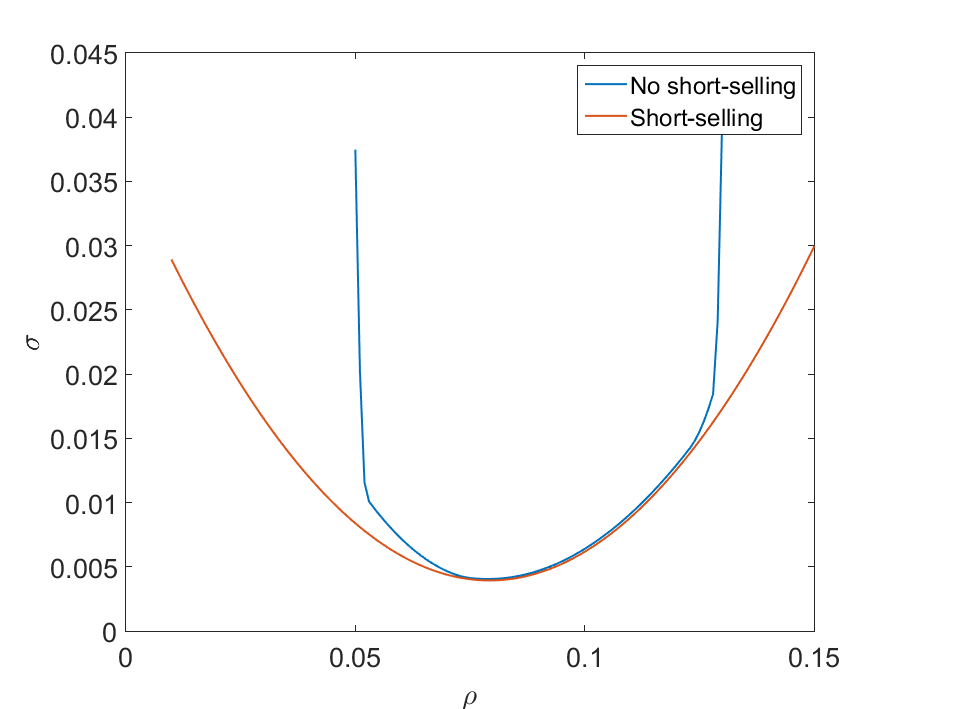
\includegraphics[width=1.0\textwidth]{../plots/r_sigma}
\end{frame}

\begin{frame}{Minimum Target Returns}
  \centering
  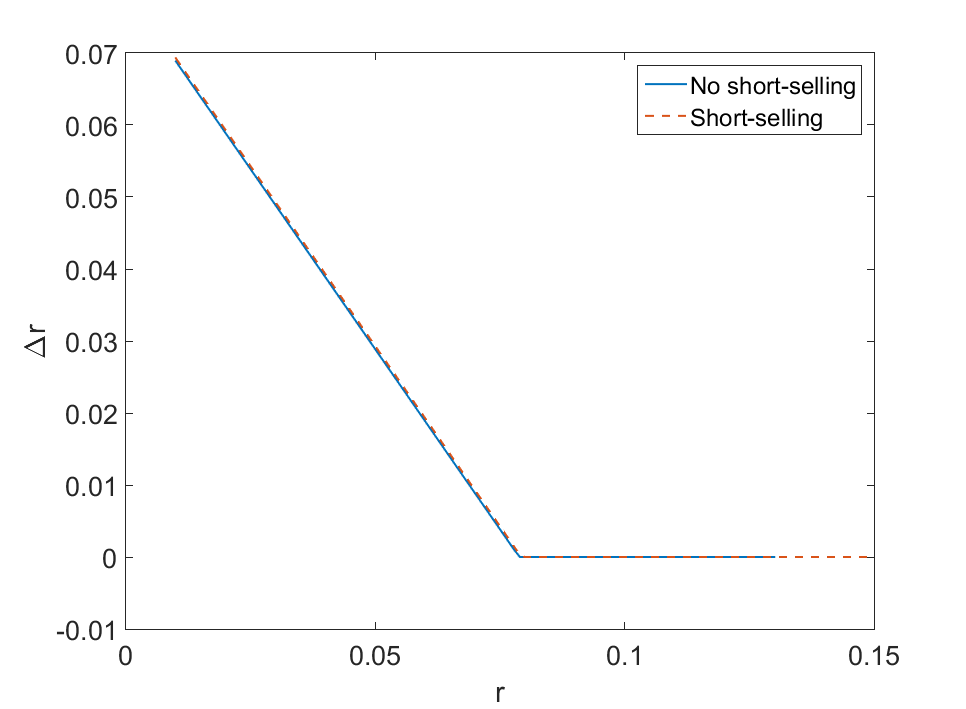
\includegraphics[width=1.0\textwidth]{../plots/delta_r}
\end{frame}

\begin{frame}{Balancing Volatility & Returns}
  \begin{itemize}
    \item{Want to balance volatility with expected returns}
    \item{Minimize $\alpha \vec w^T \boldsymbol{\sigma} \vec w - (1-\alpha)\vec r$ for $\alpha \in [0, 1]$ instead.}
    \begin{itemize}
      \item{$\alpha = 1 \to$ minimize volatility.}
      \item{$\alpha = 0 \to$ maximize profit.}
    \end{itemize}
    \item{Solving for different values of $\alpha$ gives a graph of $\bar r$ vs. $\bar \sigma$ called the efficient frontier.}
  \end{itemize}
\end{frame}

\begin{frame}{$\bar r$ vs $\bar \sigma$ (no short-selling)}
  \centering
  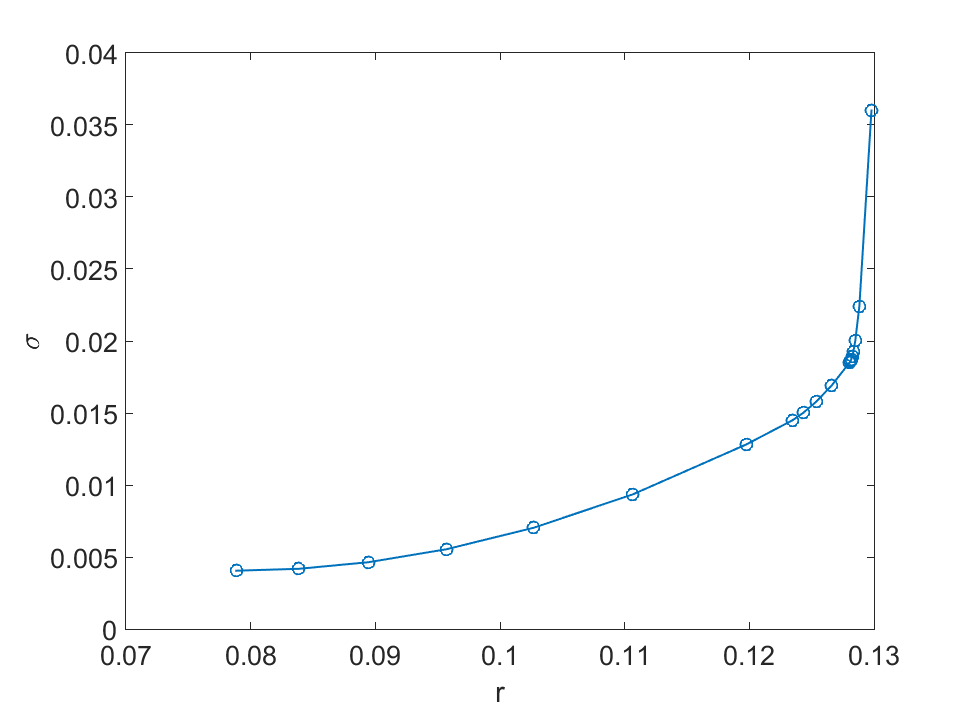
\includegraphics[width=1.0\textwidth]{../plots/r_sigma_alpha_no_ss}
\end{frame}

\begin{frame}{$\bar r$ vs $\bar \sigma$ (with short-selling)}
  \centering
  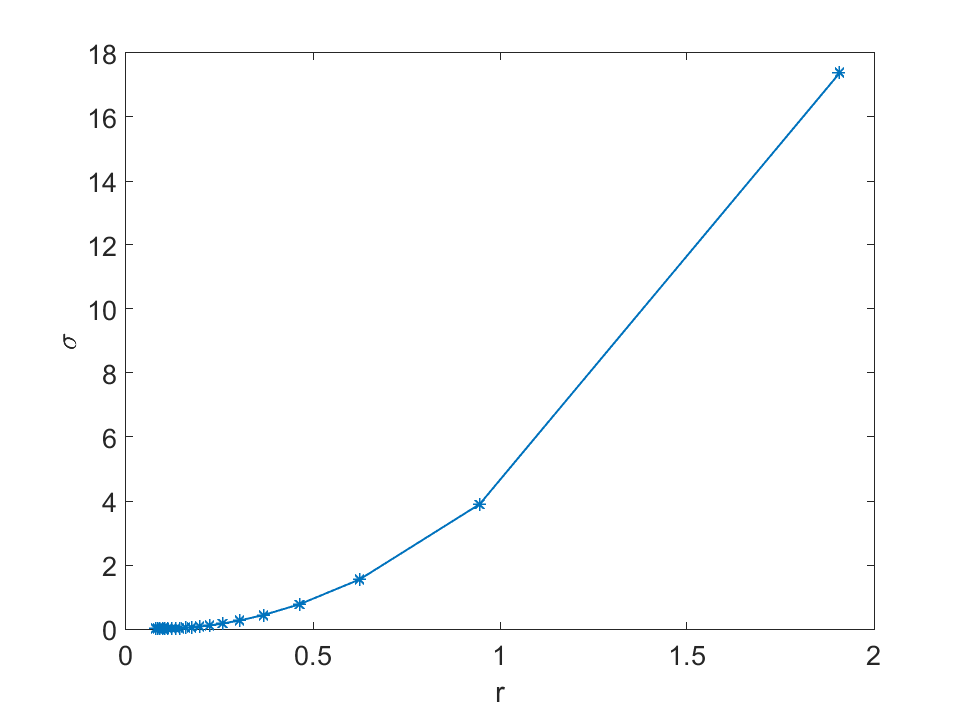
\includegraphics[width=1.0\textwidth]{../plots/r_sigma_alpha_ss}
\end{frame}

\begin{frame}
  \Huge\centering
  Any Questions?
\end{frame}

\end{document}
